\section{Глобальная погрешность. Устойчивость метода. Ограничение на шаг. Явление жесткости и методы решения жестких систем.}\label{sec:ch27}
Подменяя анализ глобальной погрешности анализом локальной, мы высказывали непременное условие такой замены --
обеспечение устойчивости решения разностного уравнения метода, которая, в свою очередь, зависит не только от формулы
метода, но и от шага интегрирования. В отсутствие возможности оценить глобальную погрешность и устойчивость метода
в общем случае появляется желание выбрать некоторую простую модельную (<<тестовую>>) систему уравнений и рассмотреть,
как формируется глобальная погрешность для нее.

Такой тестовый пример должен удовлетворять двум требованиям. С одной стороны, он должен быть достаточно простым,
чтобы можно было выполнить необходимый анализ, а с другой стороны, он должен быть достаточно <<представительным>> в
том смысле, что сравнительные выводы о свойствах устойчивости различных методов должны носить относительно общий
характер и распространяться на значительный круг задач. Этим требованиям удовлетворяет система линейных уравнений
\begin{equation}
    \frac{d\bf{x}(t)}{dt} = \bf{A}\bf{x}(t) \label{eq:hard1}
\end{equation}
с постоянной матрицей. Она является достаточно представительной, так как нелинейная система может быть линеаризована
в окрестности некоторой точки решения и заменена системой~\eqref{eq:hard1}. Если какой-либо метод продемонстрирует
негативные свойства в смысле устойчивости на примере системы~\eqref{eq:hard1}, трудно ожидать от него хороших свойств
на нелинейной задаче. Обратное верно не всегда.

Пусть все собственные значения $\uplambda_k$ матрицы \bf{A} лежат в левой полуплоскости. Тогда решение системы
дифференциальных уравнений~\eqref{eq:hard1} будет асимптотически устойчиво. Чтобы численный метод адекватно отражал
реальность, необходимо потребовать, чтобы его разностное уравнение также обладало асимптотически устойчивым решением.

Первоначально обратимся к явному методу ломаных Эйлера. Его формула применительно к~\eqref{eq:hard1} записывается в виде
\begin{equation*}
    \bf{x}_{n+1} = \bf{x}_n + h\bf{f}(t_n, \bf{x}_n) = \bf{x}_n + h\bf{A}\bf{x}_n = \left( \bf{E} + h\bf{A} \right)\bf{x}_n
\end{equation*}
Для асимптотической устойчивости решения разностного уравнения необходимо, чтобы собственные значения матрицы $\bf{E} + h\bf{A}$,
равные $1 + h\uplambda_k$, по модулю были меньше единицы, что для вещественных отрицательных $\uplambda_k$ приводит
к выполнению неравенства
\begin{equation}
    -1 < 1 + h\uplambda_k < 1, \qquad h|\uplambda_k| < 2 \label{eq:hard2}
\end{equation}
Для комплексных значений $h\uplambda_k = h\alpha_k + jh\omega_k$, условие асимптотической устойчивости
\begin{equation*}
    \left( 1 + h\alpha_k \right)^2 + h^2 \omega_k^2 < 1
\end{equation*}
требует, чтобы их значения находились на комплексной плоскости внутри круга с единичным радиусом и центром $(-1, 0)$,
а ограничение на шаг имело вид:
\begin{equation*}
    h < \frac{-2\alpha_k}{\displaystyle \left( \alpha_k^2 + \omega_k^2 \right)}
\end{equation*}
\begin{definition}
    Множество решений $h\uplambda_k$, удовлетворяющих условию устойчивости разностного уравнения метода, называют
    \emph{областью устойчивости} данного метода.
\end{definition}
Для явного метода ломаных Эйлера, который является одновременно методом Адамса первой степени и методом Рунге-Кутты
первой степени, она представлена на рисунке кривой $s = 1$.
\begin{figure}[H]
    \centering
    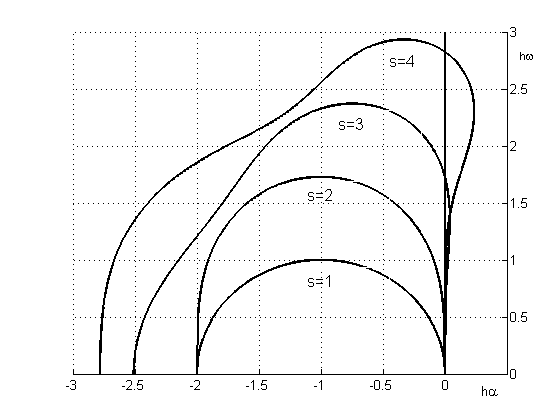
\includegraphics[width=.7\linewidth]{subfiles/images/27_1}
    \caption{Области устойчивости явных методов Рунге-Кутты}
\end{figure}

Является ли условие~\eqref{eq:hard2} недостатком только явного метода ломаных Эйлера, и как ведут себя другие
численные методы для жестких систем? К сожалению, все рассмотренные явные методы Рунге-Кутты и Адамса непригодны
для решения жестких систем. Так, последовательно применяя методы Рунге-Кутты второй, третьей и четвертой степени
к системе~\eqref{eq:hard1}, получаем следующие разностные уравнения:
\begin{flalign*}
    &\bf{x}_{n+1} = \left( \bf{E} + h\bf{A} + \frac{h^2\bf{A}^2}{2} \right)\bf{x}_n\\
    &\bf{x}_{n+1} = \left( \bf{E} + h\bf{A} + \frac{h^2\bf{A}^2}{2} + \frac{h^3\bf{A}^3}{6} \right)\bf{x}_n\\
    &\bf{x}_{n+1} = \left( \bf{E} + h\bf{A} + \frac{h^2\bf{A}^2}{2} + \frac{h^3\bf{A}^3}{6} + \frac{h^4\bf{A}^4}{24} \right)\bf{x}_n
\end{flalign*}
и ограничения на шаг интегрирования, подобно~\eqref{eq:hard2} задающие области устойчивости:
\begin{flalign}
    &\left| 1 + h\uplambda + \frac{h^2\uplambda^2}{2} \right| < 1\\
    &\left| 1 + h\uplambda + \frac{h^2\uplambda^2}{2} + \frac{h^3\uplambda^3}{6} \right| < 1\\
    &\left| 1 + h\uplambda + \frac{h^2\uplambda^2}{2} + \frac{h^3\uplambda^3}{6} + \frac{h^4\uplambda^4}{24} \right| < 1
\end{flalign}
Для вещественных отрицательных $\uplambda_k$ эти ограничения принимают вид
\begin{flalign*}
    &h|\uplambda_k| < 2 \text{-- методы второй степени;}\\
    &h|\uplambda_k| < 2.513  \text{-- метод третьей степени;}\\
    &h|\uplambda_k| < 2.785 \text{-- метод Рунге-Кутты четвертой степени.}
\end{flalign*}
Для общего случая комплексных значений $\uplambda_k$ области устойчивости представлены на рисунке выше. Так как все
области обладают свойством симметрии относительно действительной оси, то воспроизводится только часть границы областей,
лежащая в верхей полуплоскости. Значения $h\uplambda_k$ внутри этих областей удовлетворяют условиям ограниченности
единицей. Хотя ограничения на шаг интегрирования незначительно ослабляются при увеличении степени метода, общий объем
вычислений при этом даже возрастает, так как растет число значений $\bf{f}(t, \bf{x})$, требуемых на каждом шаге.

Еще хуже обстоят дела с устойчивостью явных методов Адамса. Их разностные схемы приводят к еще более серьезным
ограничениям на $h$ по сравнению с методами Рунге-Кутты:
\begin{flalign*}
    &h|\uplambda_k| < 1.0 \text{-- метод Адамса второй степени;}\\
    &h|\uplambda_k| < 6/11 \text{-- метод Адамса третьей степени;}\\
    &h|\uplambda_k| < 0.3 \text{-- метод Адамса четвертой степени;}
\end{flalign*}
\begin{figure}[H]
    \centering
    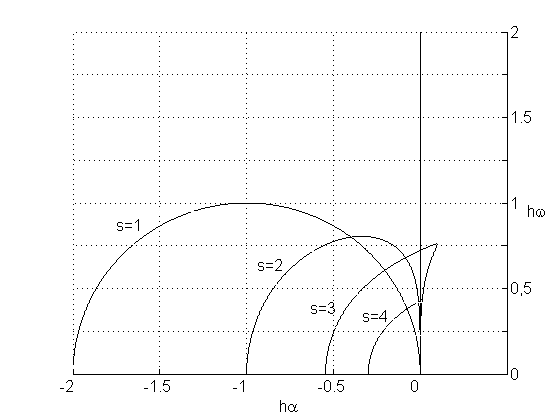
\includegraphics[width=.7\linewidth]{subfiles/images/27_2}
    \caption{Области устойчивости явных методов Адамса}
\end{figure}
Общая ситуация для вещественных отрицательных значений $\uplambda_k$ складывается следующим образом. Время наблюдения
решения $T$ определяется минимальным по модулю собственным значением матрицы \bf{A}, а шаг интегрирования -- максимальным.
Тогда число шагов $N$ прямо пропорционально числу обусловленности, что и приводит к недопустимым затратам
\begin{equation*}
    T \sim \frac{1}{|\uplambda_k|_{\text{min}}}, \qquad h \sim \frac{1}{|\uplambda_k|_{\text{max}}}, \qquad N = \frac{T}{h} \sim \frac{|\uplambda_k|_{\text{max}}}{|\uplambda_k|_{\text{min}}} \gg 1
\end{equation*}
Чтобы изменить ситуацию, для методов, предназначенных интегрировать жесткие системы, следует потребовать, чтобы их
область устойчивости включала в себя всю или почти всю левую полуплоскость, что позволит устранить ограничение на
шаг типа~\eqref{eq:hard2} и увеличить шаг, когда пограничный слой уже пройден.

Используем для решения~\eqref{eq:hard1} неявный метод ломаных Эйлера. Соответствующее разностное уравнение и
ограничение на шаг примут следующий вид:
\begin{equation*}
    \bf{x}_{n+1} = \bf{x}_n + h\bf{A}\bf{x}_{n+1} = \left( \bf{E} - h\bf{A} \right)^{-1}\bf{x}_n, \qquad |1 - h\uplambda_k| > 1
\end{equation*}
Полагая величину $\uplambda_k$ комплексной, $\uplambda_k = \alpha_k + j\omega_k$, для области устойчивости метода (рис. 3)
получим:
\begin{equation*}
    \left( 1 - h\alpha_k \right)^2 + h^2 \omega_k^2 > 1
\end{equation*}
Она включает в себя всю левую полуплоскость, и неустойчивость метода проявляется только в круге единичного радиуса с
центром в точке $(1, 0)$.
\begin{figure}[H]
    \centering
    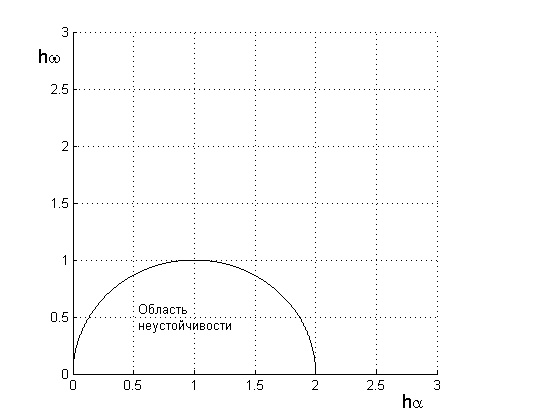
\includegraphics[width=.7\linewidth]{subfiles/images/27_3}
    \caption{Области устойчивости неявного метода ломаных Эйлера}
\end{figure}
Еще более интересный результат наблюдаем для неявного метода трапеций
\begin{gather*}
    \bf{x}_{n+1} = \bf{x}_n + \frac{h}{2}\left( \bf{A}\bf{x}_{n+1} + \bf{A}\bf{x}_n \right), \qquad \left( \bf{E} - \frac{h}{2}\bf{A} \right)\bf{x}_{n+1} = \left( \bf{E} + \frac{h}{2}\bf{A} \right)\bf{x}_n \\
    \bf{x}_{n+1} = \left( \bf{E} - \frac{h}{2}\bf{A} \right)^{-1} \left( \bf{E} + \frac{h}{2}\bf{A} \right)\bf{x}_n, \qquad \left| \frac{1 + h\uplambda_k/2}{1 - h\uplambda_k/2} \right| < 1
\end{gather*}
Тогда для $\uplambda_k = \alpha_k + j\omega_k$ получаем
\begin{equation*}
    \left( 1 + \frac{h\alpha}{2} \right)^2 + \frac{h^2 \omega^2}{4} < \left( 1 - \frac{h\alpha}{2} \right)^2 + \frac{h^2 \omega^2}{4}
\end{equation*}
что после упрощений приводит к выполнению неравенства $h\alpha < 0$, т.е. область устойчивости метода совпадает с
областью, где устойчивость имеет место для решения дифференциального уравнения. Таким образом, оба алгоритма могут
быть рекомендованы для решения жестких систем. Как будет видно ниже, типичное для неявных методов некоторое увеличение
трудоемкости одного шага интегрирования с лихвой окупается большим выигрышем в величине шага для жестких систем.
